\chapter{Evaluierung}

Die Qualität der Ergebnisse des in der Implementierung realisierten Modells wird in diesem Kapitel durch ein Testexperiment überprüft. Weiterhin werden Ausführungszeiten für beispielsweise verschieden große $k$ beim Bag of Visual Words betrachtet, um eine Einsicht in die Performance der Algorithmen zu gewinnen.
Im Kapitel Experimentaufbau wird zunächst das Experiement sowie verwendete Metriken und Ergebnistypen behandelt. Nachfolgend wird erläutert, wie die großen Menge an benötigten Trainings- und Testdaten wiederholbar und automatisiert aufgebaut wird. Dieser Abschnitt illustriert auch, wie eine Durchführung des Experiments vonstatten geht. Im letzten Teil werden dann konkrete Testgruppen aus den Caltech101 \cite{cal2004} Bilddaten erzeugt. Diese Menge an Bilddaten hat große Verbreitung im Bereich der Objekterkennung gefunden. Auf diese Weise ist ein Vergleich mit Arbeiten Anderer prinzipiell möglich.

\section{Testdaten und Testgenerierung}

Der Abschnitt Testdaten stellt die hier verwendete Menge von Bildern vor, die Caltech101, welche extra für den Test von Algorithmen bezüglich der Objekterkennung in Bildern entwickelt wurde.\newline
Im folgenden Abschnitt zur Testgenerierung wird ein Verfahren zur zufälligen Auswahl von Trainings- und Testbildern unter Berücksichtigung verschiedener Restriktionen, wie z.B. dem Verhältnis der Anzahl von Trainings- zu Testbildern vorgestellt.

\subsection{Testdaten}

Als Testmenge wurden die Bilder der Caltech101-Menge verwendet. Bei Caltech101 handelt es sich um eine weit verbreitete Menge von Bilddaten, die vorwiegend zum Test von Algorithmen bezüglich der Objekterkennung in Bildern dient. Insgesamt liegen, wie der Name sagt, 101 Kategorien vor, die jeweils zwischen 40 und 800 Bildern enthalten. Auf der offiziellen Webseite \footnote{http://www.vision.caltech.edu/Image\textunderscore Datasets/Caltech101/} und im Artikel der Autoren wird empfohlen, die eigene Arbeit mit derer anderen vergleichbar zu halten, indem:

\begin{itemize}
	\item Eine feste Anzahl an Trainings- und Testbildern verwendet wird.
	\item Experimente mit einer zufälligen Auswahl an Bildern wiederholt werden.
	\item Ähnlich viele Bilder, wie in den Arbeiten anderer, verwendet werden (1, 3, 5, 10, 15, 20 oder 30 Trainingsbilder; 20 oder 30 Testbilder).
\end{itemize}

Die Caltech101 Daten liegen nach Download kategorisiert im JPG-Format vor. Die Struktur wurde so beibehalten und ist noch für die Testgenerierung relevant. Direkt unter dem Caltech101-Ordner ist pro Kategorie ein Ordner vorhanden, der die jeweiligen Bilder immer im gleichen Namensschema enthält:\newline

\dirtree{%src
.1 Caltech101.
.2 accordion.
.3 image\textunderscore 0001.jpg.
.3 image\textunderscore 0002.jpg.
.3 ....
.2 airplanes.
.3 ....
.2 ....
}

Abbildung \ref{img:strawberries} zeigt vier Bilder aus der Kategorie \enquote{Erdbeere}. Neben Bildern von realen Rosengewächsen sind auch Zeichnungen und Objekte enthalten, die Form und Farbe der Erdbeere nachempfunden sind. Auch sind die Objekte auf einem Bild zum Teil in unterschiedlicher Menge vorhanden. Durch diese Variation ist ein Algorithmus so gefordert, tatsächlich eine Abstraktion zu lernen.

\begin{figure}
	\centering
	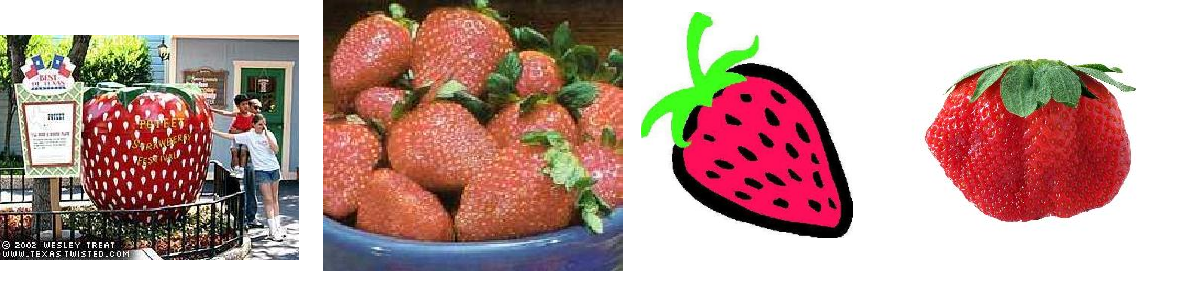
\includegraphics[scale=0.5]{images/strawberry.png}
	\caption{Verschiedene Bilder aus der Kategorie \enquote{Erdbeere} der Caltech101 Bilddaten.}
	\label{img:strawberries}
\end{figure}

\subsection{Testgenerierung}

Die Generierung von Testdaten bietet sich aus mehreren Gründen an. Zum einen sind enorm viele Trainingsdaten notwendig, um ein leistungsfähiges Modell zu generieren, zum anderen sollen im Test ca. 2000 Bildpaare verwendet werden. Ein manueller Testaufbau wäre fehleranfällig und nicht sehr flexibel. Da ein praktisch taugliches Modell erst durch die Variation einiger Parameter gefunden werden kann, ist es wünschenswert, Testdaten mit verschiedenen Eigenschaften generieren zu können:

\begin{itemize}
	\item Die Anzahl der Kategorien sollte bestimmbar sein. Dies entspricht einer Kategorie der Caltech101-Daten. Somit sind hier theoretisch bis zu 101 Kategorien im Test denkbar.
	\item Das Verhältnis bzw. die Anzahl an Trainings- und Testbildern muss definierbar sein.
\end{itemize}

Letztendlich sollen die Histogramme der \textit{Visual Words} zweier Bilder miteinander verglichen und so die Ähnlichkeit gemessen werden. Ein Programm automatisiert daher die Generierung solcher Paare: Es werden zufällige Bildpaare aus ausgewählten Kategorien (\textit{airplanes}, \textit{anchor}, ...) selektiert. Diese Paare, sowie die Information, ob die Bilder in der selben oder einer verschiedenen Kategorie liegen, stellen einen Testkandidaten dar. Zwei Bilder liegen dabei in der selben Klasse, wenn sie im selben Ordner im Dateisystem, also hier im Caltech101-Ordner, enthalten sind. Das Ergebnis wird dann als Datei \textit{test \textunderscore time.txt} gespeichert. Die Pfade der Bilder werden hierbei relativ zum Caltech101-Ordner gespeichert, die Information über die Kategorie wird als \enquote{+} bzw. \enquote{-} kodiert. Eine Datei für die Kategorien \textit{airplanes} und \textit{anchor} könnte dann so beginnen:\newline

\begin{lstlisting}
airplanes/image_0023.jpg airplanes/image_0009.jpg +
airplanes/image_0002.jpg anchor/image_0015.jpg -
anchor/image_0013.jpg airplanes/image_0002.jpg -
anchor/image_0001.jpg anchor/image_0005.jpg +
airplanes/image_0006.jpg anchor/image_0006.jpg -
...
\end{lstlisting}

Neben den zu verwendenden Kategorien muss bei Erzeugung die Anzahl der Testkandidaten, das Verhältnis von positiven zu negativen Kategorien sowie die Anzahl der Trainings- und Testbilder angegeben werden. \newline
Die Bilder, welche durch das Programm für das Training ausgewählt wurden, werden separat als \textit{train\textunderscore time.txt} gespeichert. Pro Zeile ist hier der relative Pfad des Bildes innerhalb des Caltech101-Ordners enthalten.

\section{Experimentaufbau}

Das Experiment soll sowohl die Feature-Kompression durch einen Autoencoder testen als auch die Kategorisierung bzw. den Vergleich der Bilder durch den Bag of Visual Words. Aus diesem Grund ist das Experiment zweigeteilt: 

\begin{enumerate}[(a)]%
	\item In dieser Variante findet ein reiner Test des Bag of Visual Words statt. Hierfür werden durch SIFT die Feature-Deskriptoren von Trainingsbildern extrahiert und direkt als Eingabe an den Bag of Visual Words gegeben. Anschließend folgt die Verarbeitung der Testbilder.
	\item Hier wird nach Extraktion der \textit{keypoints} durch den SIFT-Detektor der Feature-Deskriptor durch den Autoencoder erzeugt. Die so erhaltenen Features werden dann wie in (a) durch den Bag of Visual Words gruppiert und anschließend die \textit{Visual Words} der Testbilder erzeugt.
\end{enumerate}

Wichtig ist, dass pro Durchführung des Experiments in beiden Varianten die gleichen Trainings- und Testbilder verwendet werden, damit die Ergebnisse beider Deskriptoren miteinander vergleichbar sind. \newline
Nach Erzeugung des Modells mit den Trainingsbildern, werden nun die Features der Testkandidaten extrahiert und pro Bild dies \textit{Visual Words} berechnet. Die Ähnlichkeit \textit{sim (similarity)} der resultierenden Histogramme $h_1$ und $h_2$ wird dann als 1 $-$ \textit{MSE (mean squared error)} gemessen:

$$sim(h_1, h_2) = 1 - MSE(h_1, h_2)$$
$$MSE(h_1, h_2) = \frac{1}{n}\sum_{i=0}^{n}(h_{1_i} - h_{2_i})^{2}$$

Beträgt die Ähnlichkeit von zwei Histogrammen 1 werden sie als identisch angesehen. Werte nahe 0 drücken aus, dass die Histogramme sich sehr voneinander unterscheiden. Damit nun unterschieden werden kann, ob zwei Bilder in derselben Klasse sind, muss die Ähnlichkeit mit einem Schwellwert verglichen werden. So kann beispielsweise definiert werden, dass es sich bei einer Ähnlichkeit größer als $0.8$ um dieselbe Klasse handelt. Somit hat der Schwellwert unmittelbar Auswirkungen auf die Ergebnisse und sollte selbst Bestandteil des Experiments sein. Das Resultat eines solchen Vergleichs ist dann einer der beiden folgenden Kategorien zuzuordnen:

\begin{itemize}
	\item \textbf{True Positives (TP)} Bei \textit{True Positives} handelt es sich um zwei Bildern die entweder in der gleichen oder einer verschiedenen Klasse liegen und die Vorhersage des Modells diesbezüglich korrekt ist.
	\item \textbf{False Positives (FP)} In diesem Fall ist die Klassifizierung durch das Modell nicht korrekt: Bei gleicher Klasse wurde eine geringe Ähnlichkeit erkannt, bei verschiedenen eine Hohe.
\end{itemize}

Damit ein Modell zuverlässige Ergebnisse liefert, muss es größtenteils \textit{True Positives} erkennen, bzw. der Anteil der \textit{True Positives} sollte im Verhältnis zu den \textit{False Positives} bei weitem überwiegen. Für eine visuelle Darstellung dieses Verhältnisses eignet sich die \textit{Receiver Operating Characteristic (ROC)}: Diese stellt die \textit{TP} auf der Ordinate und die \textit{FP} auf der Abzisse dar.

\section{Experimentdurchführung}

Das Clustering wurde in drei Experimenten getestet. Pro Experiment wurden Eigenschaften einer Bildmenge variiert, um zu beobachten, wie sich diese Veränderungen auf die Qualität der Ergebnisse auswirkt. Die Testmengen sind jeweils wie folgt gewählt:

\begin{itemize}
	\item \textbf{Test 1} besteht aus zwei Kategorien: \enquote{Bonsai} und \enquote{Leopard}. Es wurden 50 Bilder verwendet, aus beiden Kategorien je 25. Von diesen Bildern sind 30\% für die Trainings- und die anderen 70\% für die Testphase bestimmt. Im Training liegen ca. $10.000$ Features vor, im Test knapp $27.000$.
	\item \textbf{Test 2} enthält ebenfalls, wie Test 1, die Kategorien \enquote{Bonsai} und \enquote{Leopard}. Hier werden aber insgesamt 100 Bilder verwendet. Aus beiden Kategorien wurden wieder gleich viele Bilder gewählt und die Aufteilung in Trainings- bzw. Testdaten bleibt auch gleich. Hier wurden für das Training ca. $21.000$ Features extrahiert und für den Test $55.000$.
	\item \textbf{Test 3} enthält drei Kategorien von Bildern, um zu testen, ob eine komplexere Kategorisierung prinzipiell möglich ist. Als Kategorien wurden hier \enquote{Flugzeug}, \enquote{Motorrad} und \enquote{Armbanduhr} gewählt. Insgesamt werden 80 Bilder verwendet, jede Kategorie steuert ein Drittel der Bilder bei. Die Aufteilung in Trainings- und Testdaten wird auch hier beibehalten. In der Trainingsphase lagen ungefähr $18.000$ Features vor, in der Testphase ca. $52.000$.
\end{itemize} 

Als Grafikkarte für die Experimente wurde eine Nvidia Quadro M4000 (GM204GL) verwendet. Bei dieser Grafikkarte stehen 48kB \textit{shared memory} zur Verfügung, sodass bei 1024 Threads 91 Cluster für SIFT und ca. 300 Cluster für die Autoencoder-Features möglich sind. Die Programme wurden unter CUDA 7.5 ausgeführt.\newline

\subsection{Qualität der Ergebnisse}

\begin{figure}
	\centering
	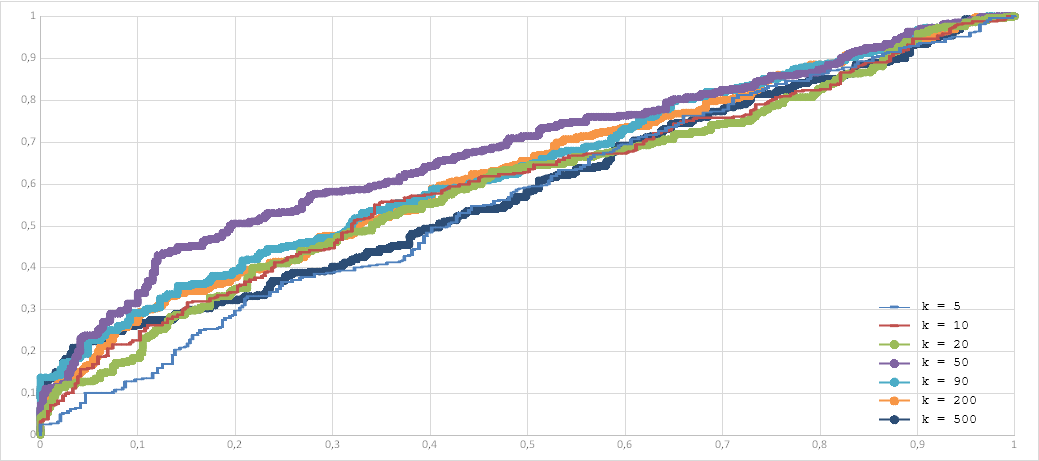
\includegraphics[scale=0.56]{images/exp1_roc128.png}
	\caption{ROC-Kurven für die SIFT-Features und verschiedene $k$ aus Experiment 1.}
	\label{img:roc1}
\end{figure}

\begin{figure}
	\centering
	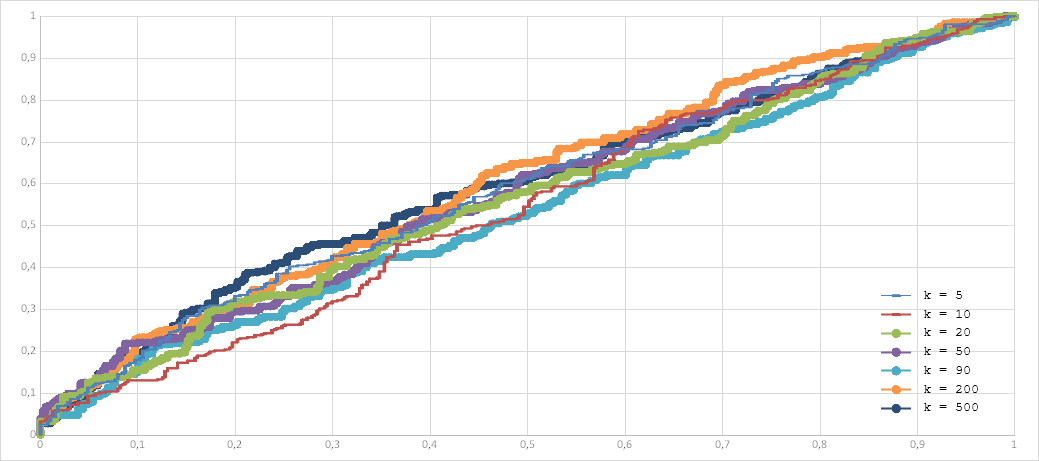
\includegraphics[scale=0.56]{images/exp1_roc36.png}
	\caption{ROC-Kurven für die Autoencoder-Features und verschiedene $k$ aus Experiment 1.}
	\label{img:roc2}
\end{figure}

\begin{figure}
	\centering
	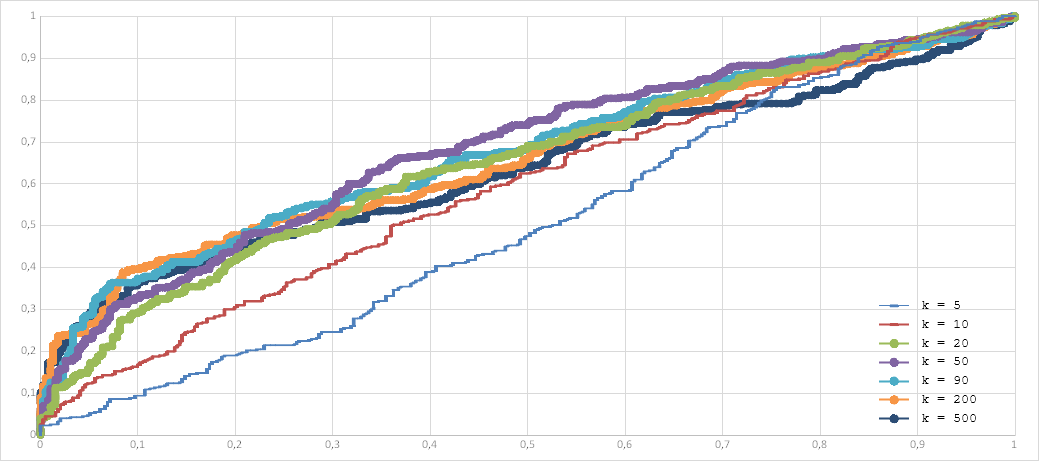
\includegraphics[scale=0.56]{images/exp2_roc128.png}
	\caption{ROC-Kurven für die SIFT-Features und verschiedene $k$ aus Experiment 2.}
	\label{img:roc3}
\end{figure}

\begin{figure}
	\centering
	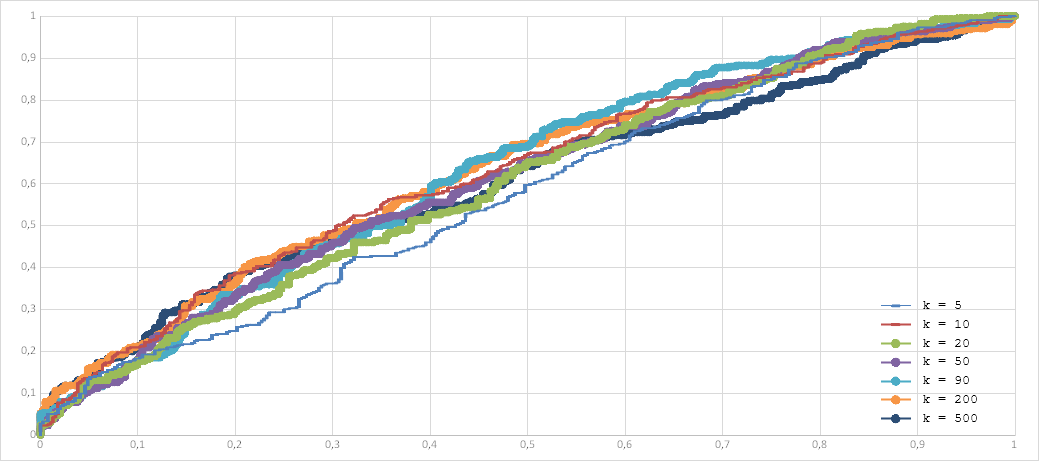
\includegraphics[scale=0.56]{images/exp2_roc36.png}
	\caption{ROC-Kurven für die Autoencoder-Features und verschiedene $k$ aus Experiment 2.}
	\label{img:roc4}
\end{figure}

\begin{figure}
	\centering
	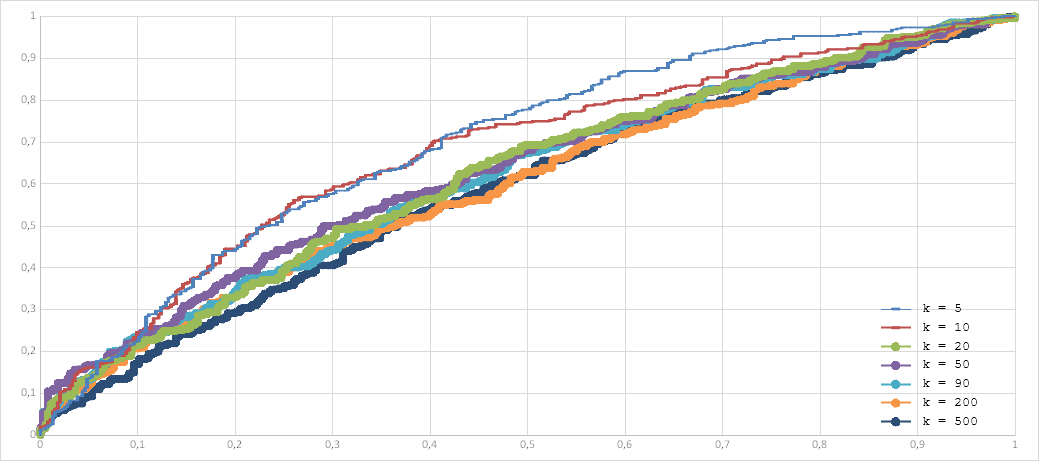
\includegraphics[scale=0.56]{images/exp3_roc128.png}
	\caption{ROC-Kurven für die SIFT-Features und verschiedene $k$ aus Experiment 3.}
	\label{img:roc5}
\end{figure}

\begin{figure}
	\centering
    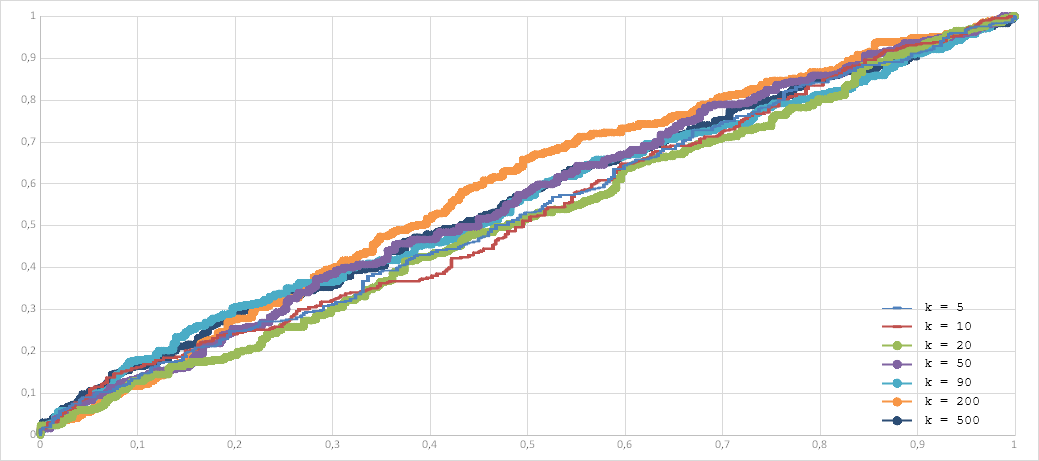
\includegraphics[scale=0.56]{images/exp3_roc36.png}
    \caption{ROC-Kurven für die Autoencoder-Features und verschiedene $k$ aus Experiment 3.}
    \label{img:roc6}
\end{figure}

% \multicolumn{2}{|c|}{Experiment 1} & \multicolumn{2}{|c|}{Experiment 2} & \multicolumn{2}{|c|}{Experiment 3}

\begin{table}
\centering

\begin{tabular}[t]{|r|r|r|r|r|r|r|}
	\hline
       & \multicolumn{2}{|c|}{Experiment 1} & \multicolumn{2}{|c|}{Experiment 2} & \multicolumn{2}{|c|}{Experiment 3} \\ \hline
      k & SIFT    & AE      & SIFT    & AE      & SIFT    & AE      \\ \hline     
      5 & 56.73 & 58.50 & 50.49 & 57.68 & \textbf{69.65} & 53.12 \\ \hline
     10 & 60.43 & 54.56 & 58.56 & 62.99 & 67.81 & 52.74 \\ \hline
  	 20 & 59.62 & 56.37 & 64.91 & 60.34 & 62.29 & 51.37 \\ \hline
 	 50 & \textbf{67.70} & 57.78 & \textbf{68.31} & 61.52 & 63.18 & 55.62 \\ \hline
	 90 & 63.59 & 53.62 & 67.47 & 63.19 & 61.77 & 55.11 \\ \hline
	200 & 62.80 & \textbf{60.49} & 66.04 & \textbf{63.24} & 60.02 & \textbf{58.17} \\ \hline
	500 & 58.90 & 59.56 & 63.39 & 60.70 & 58.84 & 55.67 \\ \hline
\end{tabular}
\caption{\textit{Area Under Curve (AUC)} der ROC-Kurven in Prozent für alle drei Experimente.}
\label{tab:AUC}
\end{table}

Für die Experimente ist in den Abbildungen \ref{img:roc1} bis \ref{img:roc6} das Ergebnis der Klassifizierung der SIFT- und Autoencoder-Features dargestellt. Hierbei handelt es sich um die \textit{global memory} Varianten. Die Werte der \textit{shared memory} Versionen sind die Gleichen, soweit diese erfasst werden konnten (bei SIFT sind maximal 90 Cluster und bei den Autoencoder-Features maximal 326 Cluster möglich). In den Grafiken wird das Verhältnis der richtig erkannten Kategorien (\textit{True Positives}) zu falsch erkannten Kategorien (\textit{False Negatives}). Hieraus ist ersichtlich, dass die Klassifizierung der SIFT- und Autoencoder-Features mäßig erfolgreich war: Ein Kurve nahe der $45${\degree} Linie sagt aus, dass das Verhältnis zwischen \textit{TP} und \textit{FP} ausgeglichen ist. In diesem Fall beträgt die Fläche unter der Kurve (\textit{Area Under Curve, AUC}) 50\%. Der \textit{AUC} für die verschiedenen Konfigurationen ist in Tabelle \ref{tab:AUC} dargestellt. Die Fläche unter der ROC-Kurve beträgt in Experiment 1 für SIFT, je nach $k$, zwischen $56.73$\% und $67.7$\%. Die Features des Autoencoders schneiden im gleichen Test meist schlechter ab. Mit einem Bestwert von $60.49$\% bei 200 Clustern, ist eine Klassifizierung nicht erfolgreich gewesen.\newline
Ein ähnliches Bild zeichnet sich bei den anderen beiden Testgruppen ab: Meist weisen die SIFT-Features eine höhere \textit{AUC} als die Autoencoder-Features auf, die Bestwerte für ein Experiment erzielen stets die SIFT-Features ($68.31$\% in Experiment 2 und $69.65$\% in Experiment 3).\newline
Auffallend ist auch, dass in Experiment 2 gegenüber Experiment 1, sowohl die Klassifizierung auf Basis der SIFT- als auch der Autoencoder-Features, erfolgreicher war. Der Aufbau beider Experimente ist recht ähnlich, nur das in Experiment zwei die doppelte Menge an Features für das Training verwendet wurde. Die Bestwerte steigen nur ein wenig ($+0.61$ für SIFT, $+2.75$ für den Autoencoder), doch die meisten Clusterkonfigurationen weisen bessere Ergebnisse auf.\newline
Überraschend ist, dass in Experiment 3 die Klassifizierung für kleine $k$, bei Verwendung der SIFT-Features, am erfolgreichsten ist ($k=5$ ist die beste Konfiguration mit $69.65$\% \textit{AUC}). Alle anderen Experimente lassen erkennen, dass eine Verwendung von $50$ bis $200$ Clustern die besten Ergebnisse liefert.\newline
Allgemein beträgt der  \textit{AUC} in allen Experimenten zwischen $50$\% und $70$\% und die Kurven verlaufen meist nah beieinander. Nur in Abbildung \ref{img:roc4} ist zu erkennen, das weniger als $20$ Cluster deutlich schlechter gegenüber Modellen mit mehr Clustern abschneiden. 

\subsection{Laufzeiten}

Für alle drei Experimente wurden sowohl die Laufzeiten der \textit{global} als auch der \textit{shared memory} Implementierung gemessen. Auf diese Weise können nicht nur die Laufzeiten der verschiedenen Features (SIFT, Autoencoder) gegenübergestellt werden, sondern auch überprüft werden, ob die Verwendung von \textit{shared memory} den Algorithmus beschleunigt. Da der durch den Autoencoder erzeugt Deskriptor ca. $3.5$ mal kleiner als der SIFT-Deskriptor ist, kann ein  Die Werte sind über zehn Testläufe gemittelt. \newline
In Tabelle \ref{tab:runtimeGlobal} sind die Laufzeiten der \textit{global memory} Variante für beide Feature-Typen dargestellt. Es ist deutlich zu erkennen, dass das Clustering der Autoencoder-Features in allen Fällen, großteils sogar sehr deutlich, schneller abgeschlossen ist, als das Clustering der SIFT-Features. In Experiment 1 und 2 ist der Prozess im Schnitt $4$ mal schneller abgeschlossen, in Experiment 3 im Schnitt nur ca. $2.8$ mal schneller.
Tabelle \ref{tab:runtimeShared} zeigt die Laufzeiten der \textit{shared memory} Implementierung. Auch hier ist das Clustering der Autoencoder-Features in Experiment 1 und 2 um einen ähnlichen Faktor schneller: Das Gruppieren des SIFT-Features ist in Experiment 1 ca. $4.6$ mal langsamer, in Experiment 2 $4.5$ mal. Für verschiedene $k$ schwankt die Reduzierung der Berechnungsdauer enorm: So ist in Experiment 2 das Clustering der Autoencoder-Features für $k=20$ gerade mal $1.8$ mal schneller, für $k=50$ hingegen fast $7$ mal schneller. Auch hier ist in Experiment 3 die Berechnung nicht so stark beschleunigt worden, wie in Experiment 1 und 2. Mit einem Faktor von $3.4$ ist dies aber immer noch näher an dem erwarteten Wert von $3.5$, als Experiment 3 der \textit{global memory} Variante.

\begin{table}
    \centering
    \begin{tabular}[t]{|r|r|r|r|r|r|r|}
    \hline
	       & \multicolumn{2}{|c|}{Experiment 1} & \multicolumn{2}{|c|}{Experiment 2} & \multicolumn{2}{|c|}{Experiment 3} \\ \hline
	k    & SIFT  & AE   & SIFT   & AE    & SIFT  & AE    \\ \hline    
    5    &  1.29 & 0.51 &  3.62  &  0.78 &  1.51 &  0.57 \\ \hline
    10   &  2.57 & 0.95 &  12.44 &  3.00 &  3.45 &  1.05 \\ \hline
    20   &  7.96 & 1.70 &  10.06 &  5.19 &  7.54 &  3.08 \\ \hline
    50   & 14.41 & 2.93 &  34.13 &  4.95 & 13.05 &  5.04 \\ \hline
    90   & 15.24 & 4.22 &  52.64 &  9.78 & 28.12 &  9.46 \\ \hline
	200  & 22.30 & 4.86 &  67.24 & 14.13 & 69.52 & 12.33 \\ \hline
	500  & 37.81 & 6.52 & 100.92 & 19.87 & 72.08 & 17.44 \\ \hline
	\end{tabular}
	\caption{Laufzeiten der \textit{global memory} Implementierung des Bag of Visual Words in Sekunden.}
	\label{tab:runtimeGlobal}
\end{table}

\begin{table}
    \centering
    \begin{tabular}[t]{|r|r|r|r|r|r|r|}
    \hline
         & \multicolumn{2}{|c|}{Experiment 1} & \multicolumn{2}{|c|}{Experiment 2} & \multicolumn{2}{|c|}{Experiment 3} \\ \hline
	k    & SIFT  & AE   & SIFT   & AE    & SIFT  & AE    \\ \hline    
    5    &  1.29 & 0.45 &   3.02 &  0.76 &  1.51 &  0.57 \\ \hline
    10   &  2.58 & 0.79 &  10.27 &  2.73 &  3.41 &  1.04 \\ \hline
    20   &  7.91 & 1.37 &   8.28 &  4.68 &  7.45 &  3.04 \\ \hline
    50   & 14.34 & 2.28 &  30.66 &  4.44 & 12.95 &  5.02 \\ \hline
    90   & 15.15 & 3.23 &  46.93 &  8.54 & 26.02 &  9.39 \\ \hline
	200  & 	   - & 3.70 &      - & 12.47 & -     & 12.26 \\ \hline
	\end{tabular}
	\caption{Laufzeiten der \textit{shared memory} Implementierung des Bag of Visual Words in Sekunden.}
	\label{tab:runtimeShared}
\end{table}